\section{Parameterization of transformations}

Use \cite{spong} as reference for rotations.

\subsection{Rotations using Roll-Pitch-Yaw}

We will parametrize rotations using roll, pitch, and yaw (RPY) respectively denoted $\phi$, $\theta$, and $\psi$. These angles denote rotations about the fixed inertial frame axes as illustrated in \cref{fig:rpy-angles}. We will use the order of rotation $x-y-z$, meaning first roll about $x_{In}$, then pitch about $y_{In}$, and then yaw about $z_{In}$.

\info[inline]{inertial frame hasn't been defined yet, might be better to just call it a base frame}


\begin{figure}
    \centering
    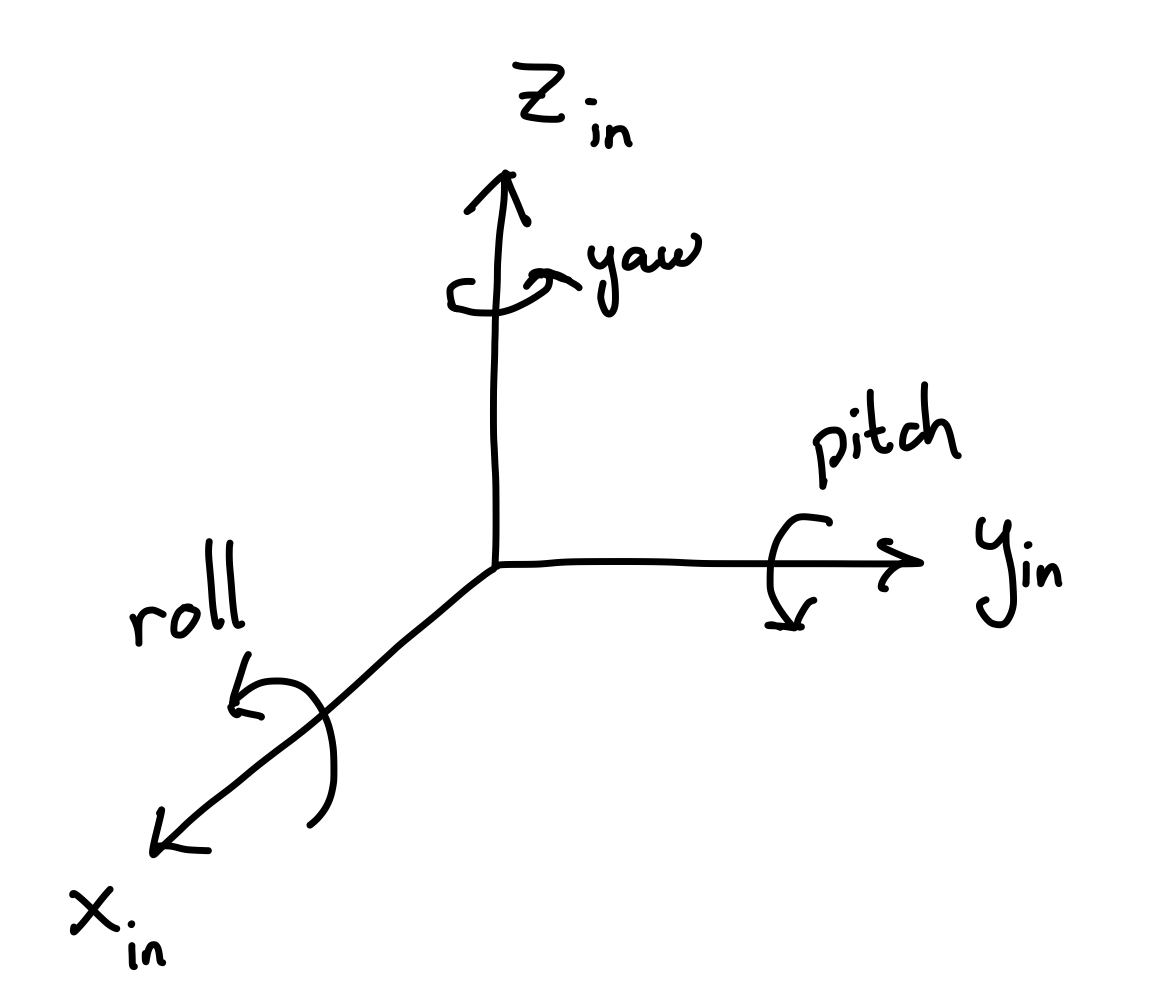
\includegraphics[width=\textwidth]{sections/figures/roll-pitch-yaw.jpeg}
    \caption{Roll-pitch-yaw angles}
    \label{fig:rpy-angles}
\end{figure}

Since we specify the RPY rotations about a fixed frame, the rotation matrix is given by

\begin{equation}
  \mathbf{R} = \mathbf{R}_{z,\psi}\mathbf{R}_{y,\theta}\mathbf{R}_{x,\phi}
\end{equation}



\subsection{Homogeneous transformations}
